\documentclass{beamer}

\usecolortheme[light]{solarized}

\beamertemplatenavigationsymbolsempty
\setbeamertemplate{frametitle}[default][center]

\usepackage{hyperref}
\usepackage{minted}

\usepackage{graphicx}
\usepackage{tikz}

\usetikzlibrary{calc, patterns}

\begin{document}

    \begin{frame}
        \begin{center}
            \Large

            Four stories: four models of learning.

            \normalsize
            \vspace{1cm}
            \href{https://twitter.com/drvinceknight}{@drvinceknight}\\
            \url{vknight.org}\\
            \texttt{knightva@cardiff.ac.uk}
        \end{center}


    \end{frame}

    \begin{frame}
        \centering

        \includegraphics[height=2cm]{static/CUident_CMYK.eps}
        \hfill
        \includegraphics[height=2cm]{static/pyconuk.jpg}
        \hfill
        \includegraphics[height=2cm]{static/axelrod_logo.png}
        \hfill
        \includegraphics[height=2cm]{static/ssi-logo.png}
    \end{frame}

    \begin{frame}
        \begin{center}
            \textbf{Active learning increases student performance in
            science, engineering, and mathematics} Freeman et al. 2014 (PNAS)
        \end{center}

        \begin{center}
            \url{https://vknight.org/tch-phi/}
        \end{center}
    \end{frame}

    \begin{frame}
        \centering
        
\includegraphics[height=.95\textheight]{static/plain/main.pdf}
    \end{frame}

    \begin{frame}
        \begin{columns}
            \begin{column}{.5\textwidth}
                \centering
                
\includegraphics[height=.45\textheight]{static/big-class/main.pdf}

                
\includegraphics[height=.45\textheight]{static/rsd/main.pdf}
            \end{column}

            \begin{column}{.5\textwidth}
                \centering
                
\includegraphics[height=.45\textheight]{static/hackathon/main.pdf}

                
\includegraphics[height=.45\textheight]{static/phd/main.pdf}
            \end{column}
        \end{columns}
    \end{frame}

    \begin{frame}
        \frametitle{First year undergraduate class}
        \centering
        
\includegraphics[height=.8\textheight]{static/big-class/main.pdf}
    \end{frame}

    \begin{frame}
        \begin{center}
            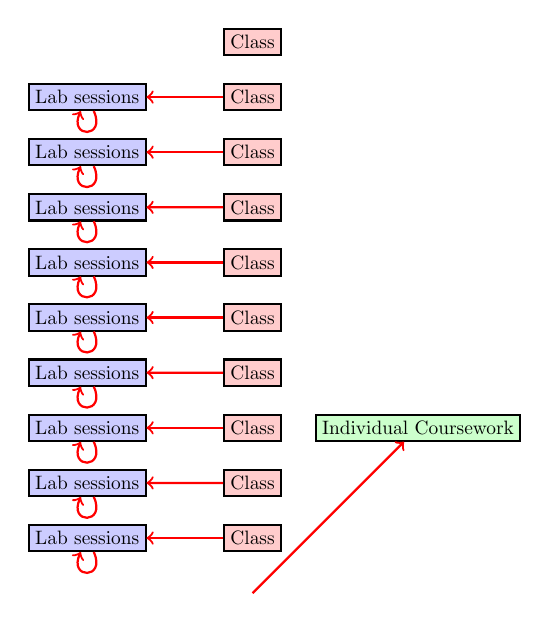
\begin{tikzpicture}[thick,scale=0.7, every node/.style={scale=0.7}]

            % Draw lab session boxes
            \node (week2) [rectangle, draw, fill=blue!20] at (0,0) {Lab sessions};
            \node (week3) [rectangle, draw, fill=blue!20] at (0,-1) {Lab sessions};
            \node (week4) [rectangle, draw, fill=blue!20] at (0,-2) {Lab sessions};
            \node (week5) [rectangle, draw, fill=blue!20] at (0,-3) {Lab sessions};
            \node (week6) [rectangle, draw, fill=blue!20] at (0,-4) {Lab sessions};
            \node (week7) [rectangle, draw, fill=blue!20] at (0,-5) {Lab sessions};
            \node (week8) [rectangle, draw, fill=blue!20] at (0,-6) {Lab sessions};
            \node (week9) [rectangle, draw, fill=blue!20] at (0,-7) {Lab sessions};
            \node (week10) [rectangle, draw, fill=blue!20] at (0,-8) {Lab sessions};
            % Draw Lecture boxes
            \node (lec1) [rectangle, draw, fill=red!20] at (3,1) {Class};
            \node (lec2) [rectangle, draw, fill=red!20] at (3,0) {Class};
            \node (lec3) [rectangle, draw, fill=red!20] at (3,-1) {Class};
            \node (lec4) [rectangle, draw, fill=red!20] at (3,-2) {Class};
            \node (lec5) [rectangle, draw, fill=red!20] at (3,-3) {Class};
            \node (lec6) [rectangle, draw, fill=red!20] at (3,-4) {Class};
            \node (lec7) [rectangle, draw, fill=red!20] at (3,-5) {Class};
            \node (lec8) [rectangle, draw, fill=red!20] at (3,-6) {Class};
            \node (lec9) [rectangle, draw, fill=red!20] at (3,-7) {Class};
            \node (lec10) [rectangle, draw, fill=red!20] at (3,-8) {Class};
            % Draw feedback arrows
            \draw [thick, red, ->] (lec2) -- (week2);
            \draw [thick, red, ->] (week2) to [out=-65, in=-115, looseness=6]  (week2);
            \draw [thick, red, ->] (lec3) -- (week3);
            \draw [thick, red, ->] (week3) to [out=-65, in=-115, looseness=6]  (week3);
            \draw [thick, red, ->] (lec4) -- (week4);
            \draw [thick, red, ->] (week4) to [out=-65, in=-115, looseness=6]  (week4);
            \draw [thick, red, ->] (lec5) -- (week5);
            \draw [thick, red, ->] (week5) to [out=-65, in=-115, looseness=6]  (week5);
            \draw [thick, red, ->] (lec6) -- (week6);
            \draw [thick, red, ->] (week6) to [out=-65, in=-115, looseness=6]  (week6);
            \draw [thick, red, ->] (lec7) -- (week7);
            \draw [thick, red, ->] (week7) to [out=-65, in=-115, looseness=6]  (week7);
            \draw [thick, red, ->] (lec8) -- (week8);
            \draw [thick, red, ->] (week8) to [out=-65, in=-115, looseness=6]  (week8);
            \draw [thick, red, ->] (lec9) -- (week9);
            \draw [thick, red, ->] (week9) to [out=-65, in=-115, looseness=6]  (week9);
            \draw [thick, red, ->] (lec10) -- (week10);
            \draw [thick, red, ->] (week10) to [out=-65, in=-115, looseness=6]  (week10);
            % Highlight assessment
            \node (ass2) [rectangle, draw, fill=green!20] at (6,-6) {Individual Coursework};
            % Feedback loops for assessment
            \draw [red, ->] (3, -9) -- (ass2);
            % ----------- Spring
            \end{tikzpicture}
        \end{center}
    \end{frame}

    \begin{frame}
        \centering
        \includegraphics[width=.9\textwidth]{static/screenshots/cfm.png}
    \end{frame}

    \begin{frame}
        \centering
        \includegraphics[width=.9\textwidth]{static/screenshots/cfm_cw.png}
    \end{frame}

    \begin{frame}
        \frametitle{Masters level 2 day hackathon}
        \centering
        
\includegraphics[height=.8\textheight]{static/hackathon/main.pdf}
    \end{frame}

    \begin{frame}
        \begin{center}
            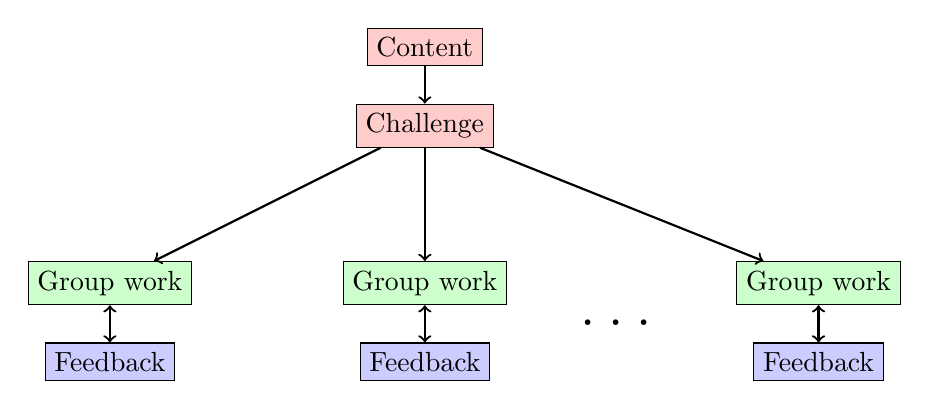
\begin{tikzpicture}
                \node (content) [rectangle, draw, fill=red!20] at (0,0)
                    {Content};
                \node (challenge) [rectangle, draw, fill=red!20] at (0,-1)
                    {Challenge};

                \node (work1) [rectangle, draw, fill=green!20] at (-4,-3)
                    {Group work};
                \node (work2) [rectangle, draw, fill=green!20] at (0,-3)
                    {Group work};
                \node (work3) [rectangle, draw, fill=green!20] at (5,-3)
                    {Group work};

                \node at (2.5, -3.5) {\Huge\dots};

                \node (feedback1) [rectangle, draw, fill=blue!20] at (-4,-4)
                    {Feedback};
                \node (feedback2) [rectangle, draw, fill=blue!20] at (0,-4)
                    {Feedback};
                \node (feedback3) [rectangle, draw, fill=blue!20] at (5,-4)
                    {Feedback};

                \draw [thick, ->] (content) -- (challenge);
                \draw [thick, ->] (challenge) -- (work1);
                \draw [thick, ->] (challenge) -- (work2);
                \draw [thick, ->] (challenge) -- (work3);

                \draw [thick, <->] (feedback1) -- (work1);
                \draw [thick, <->] (feedback2) -- (work2);
                \draw [thick, <->] (feedback3) -- (work3);
            \end{tikzpicture}
        \end{center}
    \end{frame}

    \begin{frame}
        \centering
        \includegraphics[width=.9\textwidth]{static/screenshots/oop.png}
    \end{frame}

    \begin{frame}
        \frametitle{PhD level research practice workshop}
        \centering
        
\includegraphics[height=.8\textheight]{static/rsd/main.pdf}
    \end{frame}

    \begin{frame}
        \begin{center}
            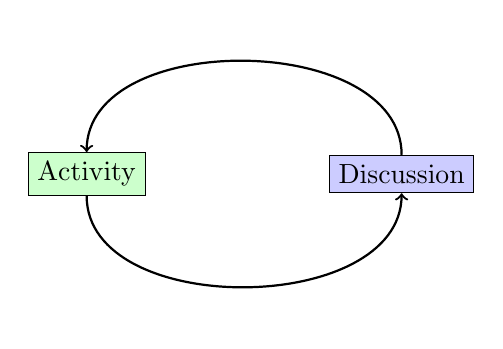
\begin{tikzpicture}
                \node (activity) [rectangle, draw, fill=green!20] at (0, 0)
                    {Activity};
                \node (discussion) [rectangle, draw, fill=blue!20] at (4, 0)
                    {Discussion};
                \draw [thick, ->] (activity) edge[out=-90, in=-90] (discussion);
                \draw [thick, ->] (discussion) edge[out=90, in=90] (activity);
            \end{tikzpicture}
        \end{center}
    \end{frame}

    \begin{frame}
        \centering
        \includegraphics[width=.9\textwidth]{static/screenshots/rsd.png}
    \end{frame}

    \begin{frame}
        \frametitle{PhD supervision}
        \centering
        
\includegraphics[height=.8\textheight]{static/phd/main.pdf}
    \end{frame}

    \begin{frame}
        \begin{center}
            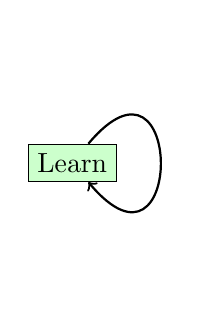
\begin{tikzpicture}
                \node (learn) [rectangle, draw, fill=green!20] at (0, 0)
                    {Learn};
                \draw [thick, ->] (learn) edge [out=50, in=-50, looseness=10] (learn);
            \end{tikzpicture}
        \end{center}
    \end{frame}

    \begin{frame}
        \begin{center}
        \includegraphics[width=.8\textwidth]{static/geraint.jpg}\\
        \end{center}
    \end{frame}

    \begin{frame}
        \begin{center}
            \includegraphics[width=.8\textwidth]{static/nik_and_i.jpg}\\
        \end{center}
    \end{frame}

    \begin{frame}
        \begin{center}
                \includegraphics[height=.95\textheight]{static/whiteboard.jpg}\\
        \end{center}
    \end{frame}

    \begin{frame}
        \begin{columns}
            \begin{column}{.5\textwidth}
                \centering
                
\includegraphics[height=.45\textheight]{static/big-class/main.pdf}

                
\includegraphics[height=.45\textheight]{static/rsd/main.pdf}
            \end{column}

            \begin{column}{.5\textwidth}
                \centering
                
\includegraphics[height=.45\textheight]{static/hackathon/main.pdf}

                
\includegraphics[height=.45\textheight]{static/phd/main.pdf}
            \end{column}
        \end{columns}
    \end{frame}

    \begin{frame}
        \centering
        \Huge Enthusiasm
    \end{frame}

    \begin{frame}

            \begin{itemize}
                \item Anaconda
                \item Jupyter notebooks
                \item \mintinline{bash}{pip install --user <package>} 
                \item gh-pages
                \item \href{https://twitter.com/drvinceknight}{@drvinceknight}
                \item \texttt{knightva@cf.ac.uk}
            \end{itemize}
    \end{frame}

\end{document}
